\documentclass[11pt, a4paper]{article}

\usepackage[utf8]{inputenc}
\usepackage[russian]{babel}
\parindent 0pt
\parskip 8pt
\usepackage{amsmath}
\usepackage{amssymb}
\usepackage{array}
\usepackage{floatrow}
\usepackage{float}
\usepackage[left=2.3cm, right=2.3cm, top=2.7cm, bottom=2.7cm, bindingoffset=0cm]{geometry}
\usepackage{hyperref}
\usepackage{graphicx}
\usepackage{multicol}
\usepackage{listings}
\usepackage{fancyhdr}
\usepackage{extramarks}
\usepackage[usenames,dvipsnames]{color}
\usepackage{titlesec}
\usepackage{tikz}
\usepackage[T2A]{fontenc}
\definecolor{grey}{RGB}{128,128,128}

\pagestyle{fancy}
\fancyhf{}
\chead{Applied Mathematics}
\rhead{\thepage}
\lfoot{by fadyat}
\cfoot{}
\rfoot{09.12.2022}
\renewcommand\headrulewidth{0.4pt}
\renewcommand\footrulewidth{0.4pt}

\begin{document}
    \begin{titlepage}
        \begin{center}
            \vspace*{2cm}
            \Large
            \textbf{Applied Mathematics}

            \vspace{1cm}
            \large
            Laboratory work №2

            \vspace{1cm}
            \textbf{Simplex method for solving linear programming problems}

            \vspace{1cm}
            \textbf{Author:} Artyom Fadeyev, Sergo Elizbarashvili
        \end{center}
    \end{titlepage}
    \newpage


    \section{Матричные игры}\label{sec:matrix_games}

    \textbf{Игра} -- это идеализированная математическая модель колективного поведения
    нескольких лиц, интересы которых различны, что приводит к конфликту.

    \textbf{Теория игр} -- это математическая теория конфликтных ситуаций, в которых
    участники принимают решения, которые влияют на их выигрыш или проигрыш.

    \textbf{Цель теории игр} -- выработка рекомендаций по разумному поведению участников
    конфликта, которые позволят им достичь наибольшего выигрыша (определить оптимальную стратегию).

    \textbf{Ходы:}
    \begin{enumerate}
        \item \textbf{Личные} -- разумное поведение участника игры, которое позволяет ему достичь наибольшего выигрыша.
        \item \textbf{Случайные} -- рандомные действия, которые принимает каждый игрок в отдельности.
    \end{enumerate}

    \textbf{Стратегия} -- совокупность правил, по которым игрок будет действовать при каждом личном ходе,
    в зависимости от ситуации в игре.

    \textbf{Оптимальная стратегия} -- стратегия, которая обеспечивает игру максимально возможный средний выигрыш или
    минимально возможный средний проигрыш, независимо от стратегии соперника.

    \textbf{Матричная игра} -- конечная парная игра с нулевой суммой, то есть в ней конечное количество ходов,
    два игрока и выигрыш одного игрока равен проигрышу другого.

    Выигрыш(проигрыш) выражается численно.
    В такой игре целью одного игрока будет максимизировать свой выигрыш, целью другого - минимизировать проигрыш.

    Пусть у игрока $A$ есть $n$ стратегий, а у игрока $B$ есть $m$ стратегий.
    Тогда матрица игры имеет размер $n \times m$.

    \begin{table}[h]
        \centering
        \begin{tabular}{|c|c|c|c|}
            \hline
            & \textbf{$B_i$} & \ldots & \textbf{$B_m$} \\
            \hline
            \textbf{$A_j$} & $a_{ij}$       & \ldots & $a_{im}$       \\
            \hline
            \vdots         & \vdots         & \ddots & \vdots         \\
            \hline
            \textbf{$A_n$} & $a_{nj}$       & \ldots & $a_{nm}$       \\
            \hline
        \end{tabular}
        \caption{Матрица игры}
        \label{tab:matrix}
    \end{table}

    Если такая таблица задана, то игра приведена к матричной форме.
    В некоторых заданиях требуется работать с уже приведенной формой.

    \newpage

    \subsection{Maximin-стратегия}\label{subsec:maximin-stategy}

    Первая из возможным стратегий - придерживаться принципа \textbf{максимин-стратегии}:
    первый игрок выбирает стратегию, при которой он получит максимальный из минимальных выигрышей,
    второй выбирает минимальный из максимальных проигрышей.

    Первое значени называется \textbf{нижней ценой игры}, а второе - \textbf{верхней ценой игры}.
    Если они равны, то матрица содержит \textbf{седловую точку}.

    Если каждый из противников применяет одну и ту же стратегию, то игра проходит в
    \textbf{чистой стратегии}.

    Случайная величина, значениями которой являются чистые стратегии, называется
    \textbf{смешанной стратегией} игрока.

    Задание смешанной стратегии состоит в указании тех вероятностей, с которыми
    выбираются его чистые стратегии.

    Частный случай: если все вероятности, кроме одной, равны нулю, то смешанная стратегия
    превращается в чистую.

    Пара стратегий $(A_i, B_j)$ называется \textbf{равновесной}, если никому из игроков
    не выгодно изменить свою стратегию.

    Если первый игрок применяет смешанную стратегию, то средний выигрыш первого игрока
    равен:

    \begin{equation}
        \sum_{i=1}^n \sum_{j=1}^m a_{ij} p_i q_j\label{eq:equation}
    \end{equation}

    Ожидаемый проигрыш второго игрока равен той же величине.

    Если матричная игра не имеет седловой точки, то игрок должен руководствоваться теми
    же принципами максимина.

    Формируя стратегию, первый игрок $A$ при которой он получит максимальный из минимальных выигрышей,
    второй игрок $B$ выбирает минимальный из максимальных проигрышей.

    \begin{equation}
        \max_{i} \min_{j} \sum_{i=1}^n \sum_{j=1}^m a_{ij} p_i q_j = v_A\label{eq:equation2}
    \end{equation}

    \begin{equation}
        \min_{j} \max_{i} \sum_{i=1}^n \sum_{j=1}^m a_{ij} p_i q_j = v_B\label{eq:equation3}
    \end{equation}

    \textbf{Основная теорема матричных игр} -- любая матричная игра имеет, по крайней мере,
    одно оптимальное решение, в общем случае, в смешанных стратегиях и соответствующую
    цену $v$.


    Следовательно, любая матричная игра имеет цену $v$.
    Цена игры $v$ называется -- средним выигрыш, приходящиймся на одну партию $\rightarrow$
    всегда удовлетворяет условию $v_l \le v \le v_r$.

    \subsection{Перевод матричной игры в эквивалентную задачу линейного программирования}\label{subsec:to_linear_programming}

    Предварительно нужно убедиться, что все элементы матрицы положительны.
    Чтобы этого добиться, можно прибавить необходимое число $C$, тогда цена игры увеличится на $C$,
    а оптимальные решения не изменятся.

    Найдем смешанную стратегию игрока $A$.
    Предположим, что игрок B применяет только чистые стратегии.
    В каждом случае выигрыш игрока $A$ будет не меньше чем $v$.

    \begin{equation}
        \begin{cases}
            a_{11}p_1 + a_{12}p_2 + \dots + a_{1m}p_m \ge v\\
            a_{21}p_1 + a_{22}p_2 + \dots + a_{2m}p_m \ge v\\
            \dots\\
            a_{n1}p_1 + a_{n2}p_2 + \dots + a_{nm}p_m \ge v
        \end{cases}\label{eq:equation4}
    \end{equation}

    Пусть $x_i = \frac{p_i}{v}$, тогда

    \begin{equation}
        \begin{cases}
            a_{11}x_1 + a_{12}x_2 + \dots + a_{1m}x_m \ge 1\\
            a_{21}x_1 + a_{22}x_2 + \dots + a_{2m}x_m \ge 1\\
            \dots\\
            a_{n1}x_1 + a_{n2}x_2 + \dots + a_{nm}x_m \ge 1\\
            x_i \ge 0, \forall i
        \end{cases}\label{eq:equation5}
    \end{equation}

    Так как игрок $A$ стремится максимизировать свой выигрыш, то можем
    сформулировать задачу линейного программирования:

    Найти значения $x$, такие что удовлетворяют системе ограничений
    и обращаются в минимум такую целевую функцию:

    \begin{equation}
        L(x) = \sum_{i=1}^m x_i\label{eq:equation6}
    \end{equation}

    Из решения найдем цену игры и оптимальную стратегию игрока $A$
    по формулам:

    \begin{equation}
        v = \frac{1}{\sum_{i=1}^m x_i}\label{eq:equation7}
    \end{equation}

    \begin{equation}
        p_i = x_i\cdot v, \forall i\label{eq:equation8}
    \end{equation}

    Аналогично можно найти оптимальную стратегию игрока $B$, но
    неравенства будут иметь обратный знак, а целевую функцию нужно
    будет максимизировать.
    Также матрица коэффициентов будет транспонированной.
    Такая задача называется \textit{двойственной}.

    \newpage


    \section{Решение задач}\label{sec:solve}

    \subsection{Задача 1}\label{subsec:task1}

    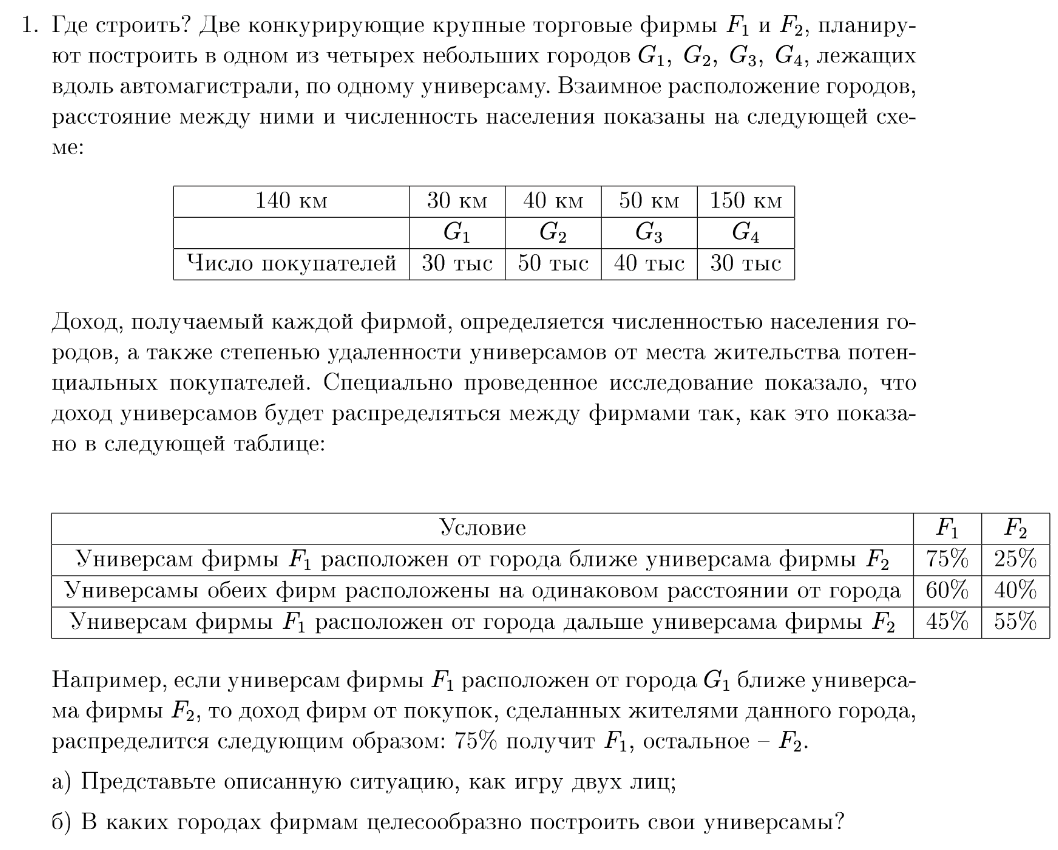
\includegraphics[width=1\textwidth]{docs/1}

    Предположим, что компания $F_1$ -- первый игрок, а $F_2$ -- второй.

    Стратегии каждого из игроков: построить универсам в городе $G_i, i = 1, 2, 3, 4$.

    Составим матрицу, в которой каждый элемент таблицы - количество тысяч человек,
    которые будут ходить в магазин первого игрока,
    если построить магазин первого игрока в городе $G_i$,
    а магазин второго игрока в городе $G_j$.

    Рассмотрим ситуацию, когда первый игрок построит магазин в городе $G_1$,
    а второй игрок в городе $G_2$.

    Посчитаем сколько людей будут ходить в магазин первого игрока:

    \begin{equation}
        30 * 0.75 + 50 * 0.45 + 40 * 0.45 + 30 * 0.45 = 76.5\label{eq:equation9}
        \text{ тыс. человек}
    \end{equation}

    Чтобы посчитать сколько людей будут ходить в магазин второго игрока нужно от 150 (население всех городов)
    отнять полученное значение для первого игрока.

    Аналогично считаем значения для всех остальных ситуаций, получаем следующую платёжную матрицу:
    \begin{table}[h]
        \centering
        \begin{tabular}{|c|c|c|c|c|c|}
            \hline
            & $G_1$ & $G_2$ & $G_3$ & $G_4$ & $\min$ \\
            \hline
            $G_1$  & 90    & 76.4  & 91.5  & 91.5  & 76.5   \\
            \hline
            $G_2$  & 103.5 & 90    & 91.5  & 103.5 & 90     \\
            \hline
            $G_3$  & 88.5  & 88.5  & 90    & 103.5 & 88.5   \\
            \hline
            $G_4$  & 88.5  & 76.5  & 76.5  & 90    & 76.5   \\
            \hline
            $\max$ & 103.5 & 90    & 91.5  & 103.5 &        \\
            \hline
        \end{tabular}\label{tab:table}
    \end{table}

    Данная игра проходит в чистых стратегиях (противники применяют одну и ту же стратегию), значит она имеет седловую точку.

    Найдем её используя принципы минимакса и максимина:

    \begin{equation}
        \max\min = \max(76.5, 90, 88.5, 76.5) = 90\label{eq:equation10}
    \end{equation}

    \begin{equation}
        \min\max = \min(103.5, 90, 91.5, 103.5) = 90\label{eq:equation11}
    \end{equation}

    Значит седловая точка игры - $(G_2, G_2)$.

    Следовательно обоим игрокам выгодно построить магазин в городе $G_2$.
    \newpage

    \subsection{Задача 2}\label{subsec:task2}
\end{document}